\documentclass[12pt]{article}
%Gumm{\color{blue}i}|065|=)
\usepackage{amsmath, amsfonts, amssymb}
\usepackage[margin=0.5in]{geometry}
\usepackage{xcolor}
\usepackage{graphicx}

% zeta funct{\color{blue}i}ons of cub{\color{blue}i}c f{\color{blue}i}elds

%\usepackage{p{\color{blue}i}font}
\usepackage{amsmath}

\newcommand{\off}[1]{}
\DeclareMathSizes{20}{30}{20}{18}

\newcommand{\two }{\sqrt[3]{2}}
\newcommand{\four}{\sqrt[3]{4}}





\usepackage{tikz}

\newcommand{\susy}{{\bf Q}}
\newcommand{\RV}{{\text{R}_\text{V}}}

\title{Scratchwork: Torus Orbits}
\date{}
\begin{document}

%\fontfam{\color{blue}i}ly{qag}\selectfont \fonts{\color{blue}i}ze{12.5}{15}\selectfont

\sffamily

\maketitle

\noindent A common step in contemprary number theory literature is to re-define the problem as a group theory problem\dots Especially using ``torus orbits".  \\ \\
Linear algebra works over any field, $K$.  So we just say ``let $K$ be a field\dots" and if we have a single plane $\mathbb{R}^m \subseteq \mathbb{R}^n$ we know more-or-less they all behave the same.  In fact, rational planes $\mathbb{Q}^m \subseteq \mathbb{Q}^n$ are not all identical.
$$ X(\mathbb{Q}) = \{ x^2 + y^2 = 1 \}  \subseteq \mathbb{Q}^2 $$
This is a $\mathbb{Q}$-torus.  Are there any rational points on this circle?  I can name $(0,\pm1)$ and $(\pm 1,0)$.  Here are two more:
$$ (\tfrac{3}{5}, \tfrac{4}{5}) , (\tfrac{5}{13}, \tfrac{12}{13}) \in X(\mathbb{Q}) $$
Since the circle was defined using algebra, we can say it is a \textbf{variety}.  In fact, $X(\mathbb{Q})$ forms a group:
$$ \left(\frac{3}{5} + i \, \frac{4}{5}\right)^2 
=  \left(\frac{3^2 - 4^2 }{25}\right) + 2 \times\left( \frac{3 \times 4}{25} \right)i =  - \frac{7}{25} + i \, \frac{24}{25}$$
Or we culd use $2 \times 2$ matrices.  There's a way find a $2 \times 2$ matrix solution to $x^2 + 1 = 0$. E.g. $(x,y) \mapsto (-y,x)$.
$$ \left[ 
\begin{array}{rr} \frac{3}{5} & -\frac{4}{5} \\  \\
\frac{4}{5} & \frac{3}{5} 
\end{array}
\right]^2 = \left[ 
\begin{array}{rr} \frac{7}{25} & -\frac{24}{25} \\ \\
\frac{24}{25} & \frac{7}{25} 
\end{array}
\right]$$
This tell us the Pythagorean triples form a \textit{multiplicative group}, but also we are looking for a $\mathbb{Q}$-action, and possibly an $\text{SL}_2(\mathbb{Z})$ action (I read it's actually a $\Gamma(2)$ action.)\\
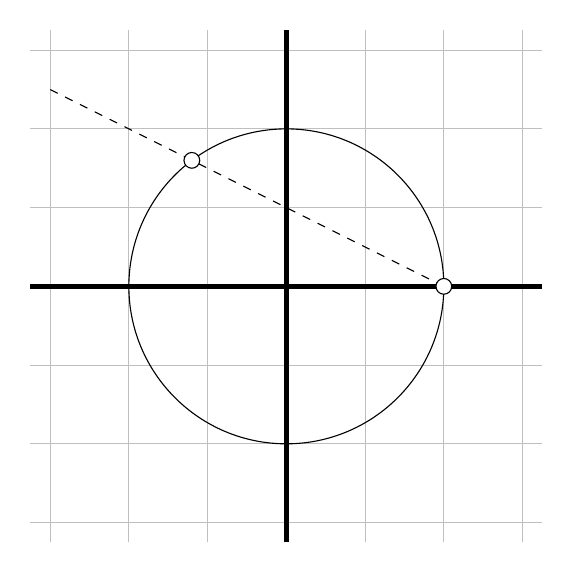
\begin{tikzpicture}
\foreach \a in {-3,...,3}{
	\draw[color=black!25!white] (\a,-3.25)--(\a,3.25);
	\draw[color=black!25!white] (-3.25,\a)--(3.25,\a);
}
\draw[color=black, line width=2] (-3.25,0)--(3.25,0);
\draw[color=black, line width=2] (0,-3.25)--(0,3.25);
\draw (0,0) circle (2);
\draw[dashed] (2,0)--(-3,2.5);
\draw[fill=white] ( 2,0) circle (0.1);
\draw[fill=white] (-1.2,1.6) circle (0.1);
\end{tikzpicture} \\
Notice we've used a tiny bit of degree theory $[circle]\cdot[line]=2 $.  This \textbf{is} an instance of cohomology\footnote{intersection theory} and we don't bother giving it a fancy name.  This is called \textbf{stereographic projection}, I think? 
\begin{eqnarray*}\big|(1,0)+ (t, mt) \big|^2 = (t+1)^2 + mt^2 &=& 1 \\
t  &=& (1,0) ,   (\tfrac{1-m^2}{m^2 + 1},- \tfrac{2m}{m^2+1}) \end{eqnarray*}
with $m = \frac{a}{b} \in \mathbb{Q}$.  These become $[a^2 - b^2 :2ab: a^2 + b^2]$ over $\mathbb{Z}$ as a proportion.  Multiplying by the slope $m \mapsto q x$ could lead to a reasonable group action of $\mathbb{Q}^\times$ on $\mathbb{Q}$. \\ \\
\textbf{Ex} Let's try solving $x^2 + y^2 + z^2 = n$ as a torus orbit of some kind.  This exercise is worked out in a handful of places.\footnote{My standard for well-known is that everybody knows it.  There are only 20000 practicing mathematicians in the US, maybe a tenth of those are number theorists.  So... } I'm going to ask for the automorphic representation $\pi$ of $\text{SL}_2(\mathbb{A})$ for a spherical harmonic $\phi \in L^2( \text{SO}_3)$.
\end{document}